\chapter{Rgb to XYZ Display simulation using a masking model}
\minitoc{}

The simulation described in this chapter corresponds to the conversion of $RGB$ to $XYZ$ tripplets using the modified masking model firstly introduced by Tamura in \cite{Tam02}.

\section{Introduction}

The basic principle of the masking model is to construct the color not only with Red, Green and Blue components, but also with secondary colors and gray. 
So the three channels (R, G and B) are simultaneously used during the measurements (given as output $X$, $Y$ and $Z$ values in $cd/m^2$). Therefore channel interaction is measured and present in the measurements. 

Therefore the 7 primary, secondary and gray curves are needed input for this simulation.

\section{Input}

\subsection{Input image}

The input image is a 24 bit RGB image saved in a raw file (64x64pixels stored as 24bit RGB).

To open it with ImageJ by instance, use "import raw file" with the following options:
\begin{itemize}
\item Image type: 24-bit RGB
\item Width: 64 pixels
\item Height: 64 pixels
\item Offset to first image: 0 bytes
\item Number of images: 1
\item Gap between images: 0
\item White is not zero
\item Little-endian byte order
\item Not open all files in folder
\item Not use virtual stack
\end{itemize}

The input image is a pink flat-field image and is shown in the figure \ref{fig:flatfieldRGB}.

\begin{figure}[!htb]
\begin{center}

\includegraphics[width=0.5\columnwidth]{./03_Rgb2XYZDisplayModule/images/pink.png}
\caption{Input pink flat-field image.}\label{fig:flatfieldRGB}
\end{center}
\end{figure}

\subsection{Input Measurements}

The 7 primary, secondary and gray curves are given as input in csv files. The first column corresponds to the digital driving level and the following columns are the $X$, $Y$ and $Z$ corresponding values. There are seven csv files, hereby a sample of the red curve:

\lstset{language=Scilab}
\begin{lstlisting}
0,0.231550150928,0.27,0.392476936462,
1,0.232805131007,0.27,0.392869413398,
2,0.235034943077,0.27,0.393262282812,
...
...
252,112.932819448,53.19,2.35753007203,
253,114.100589483,53.74,2.38192031594,
254,115.310823883,54.31,2.4071974778,
255,116.538441874,54.88,2.41509104764,
\end{lstlisting}

There are seven curves:
\begin{itemize}
\item Red: "red.csv
\item Green: "green.csv"
\item Blue: "blue.csv"
\item Cyan: "cyan.csv"
\item Magenta: "magenta.csv"
\item Yellow: "yellow.csv"
\item Gray: "gray.csv"
\end{itemize}

\section{Command}

For running the simulation, the following command is needed:

\lstset{language=C++}
\begin{lstlisting}
"..\vct\VCT.exe" SuperXML ".\xml\test_Rgb2XYZDisplayModule.xml" "."
\end{lstlisting}

The first argument is the path to the VCT executable. The second argument is simply the key word "SuperXML" and the third one is the path to the xml file. Any additional parameters are used within the xml file, in this case, it corresponds to an input path.

\section{xml}

The input xml file is:

\lstset{language=XML}
\begin{lstlisting}
<?xml version="1.0" encoding="ISO-8859-1"?>
<SuperXML>
	<LIST_OF_ITERATIONS name = "pipeline" value="1">	
	</LIST_OF_ITERATIONS>
	
	<LIST_OF_PARAMETERS>
		<LocalParameter name = "REF">
			<SequenceRawGeneratorModule name="directory" value = "#0\input"/>
		</LocalParameter>				
	</LIST_OF_PARAMETERS>

	<TEMPLATE_MEVIC_SIMULATION>
		<REF>
			<SequenceRawGeneratorModule>
				<directory dataType="char" value = "$"/>
				<number_of_slices dataType="int" value = "1"/>
				<width dataType = "int" value = "64"/>
				<height dataType = "int" value = "64"/>
				<nbBitsRange dataType = "int" value = "8"/>
				<_0bigEndian_1littleEndian dataType = "int" value = "0"/>
				<nbBitsOutput dataType = "int" value = "8"/>
				<nbBitsPrecision dataType = "int" value = "24"/>
				<_1WhiteIs0_0Otherwise dataType = "int" value = "0"/>
				<frame_repeat dataType = "int" value = "1"/>
				<_1RGB_0GRAY dataType = "int" value = "1"/>			
			</SequenceRawGeneratorModule>
			<DisplayModule>
				<_1Color_0Monochrome dataType="int" value="1"/>
				<filenameNativeCurveGray dataType="char" value = "#0\input\gray.csv"/>
				<filenameNativeCurveRed dataType="char" value = "#0\input\red.csv"/>
				<filenameNativeCurveGreen dataType="char" value = "#0\input\green.csv"/>
				<filenameNativeCurveBlue dataType="char" value = "#0\input\blue.csv"/>
				<filenameNativeCurveCyan dataType="char" value = "#0\input\cyan.csv"/>
				<filenameNativeCurveMagenta dataType="char" value = "#0\input\magenta.csv"/>
				<filenameNativeCurveYellow dataType="char" value = "#0\input\yellow.csv"/>
				<nbBits dataType="int" value="8"/>
				<frequency dataType="int" value="50"/>	
			</DisplayModule>	
			<Rgb2XYZDisplayModule>
			</Rgb2XYZDisplayModule>
			<SaveFrameTXTModule>
				<Filename dataType="char" value="#0\outputTest\init_txt"/>
				<ComponentToWrite dataType="int" value="0"/>
				<FrameToWrite dataType="int" value="-1"/>
				<ChannelToWrite dataType="int" value="-1"/>
			</SaveFrameTXTModule>	
			<SaveFrameRAWModule>
				<Filename dataType="char" value="#0\outputTest\init_raw"/>
				<ComponentToWrite dataType="int" value="0"/>
				<FrameToWrite dataType="int" value="-1"/>
				<ChannelToWrite dataType="int" value="-1"/>
			</SaveFrameRAWModule>		
			<SaveFrameTXTModule>
				<Filename dataType="char" value="#0\outputTest\txt"/>
				<ComponentToWrite dataType="int" value="1"/>
				<FrameToWrite dataType="int" value="-1"/>
				<ChannelToWrite dataType="int" value="-1"/>
			</SaveFrameTXTModule>	
			<SaveFrameRAWModule>
				<Filename dataType="char" value="#0\outputTest\raw"/>
				<ComponentToWrite dataType="int" value="1"/>
				<FrameToWrite dataType="int" value="-1"/>
				<ChannelToWrite dataType="int" value="-1"/>
			</SaveFrameRAWModule>		
		</REF>	
	</TEMPLATE_MEVIC_SIMULATION>
</SuperXML>
\end{lstlisting}

For the module "SequenceRawGeneratorModule", the character sequence "$\#0$" is replaced by the additional input argument given at the execution of the program. 

\section{Output}

The output is a an image or a sequence or XYZ frames.

\section{Module: SequenceRawGeneratorModule}

\subsection{Parameter: "directory"}

This module is used for loading an image or a sequence of images. The first parameter of this module corresponds to a path of a directory. If the directory has more than one file with the extension "raw", the module will open directly the files with the raw extension depending on the following parameter: "number\_of\_slices".

\subsection{Parameter: "number\_of\_slices"}

If this parameter is equal to "1" then only one image is opened.

\subsection{Parameter: image-sequence}

The parameters from "" to "" correspond to the image or the sequence.

\subsection{Parameter: "frame\_repeat"}

In order to generate a sequence of frames for the display simulation, this parameter can be used. If this parameter is equal to 1, one slice from the input sequence corresponds to 1 frame in the simulation. In order to repeat each slice this parameter can be used with a value superior to 1. This frame repeat parameter can be in float like described in \cite{Mar12} in order to simulate a browsing speed that is not an integer.

Let $F_{browse}$ show the slice browsing speed, F$_{refresh}$ show the frame refresh rate (a display property in $Hz$), and $FR$ show frame repeat. $F_{browse}$ = $\frac{F_{refresh}}{F}$. For example, at $F_{refresh}$ of $50$ frame per second ($fps$), if each slice is fed twice to the display at consecutive refreshes ($FR = 2$), the apparent slice browsing speed is $\frac{50}{2} = 25$ slice per second ($sps$). In other words, $FR = \frac{F_{refresh}}{F_{browse}} = \frac{50}{25} = 2$. Hence, the browsing speeds that can be simulated with integer FRs are very limited. By allowing a fractional frame repeat, one can have arbitrary browsing speeds as follows. As an example, $F_{browse}$ of $40$ $sps$ can be achieved if we make $5$ frames out of every $4$ slices. In this case $FR = \frac{F_{refresh}}{F_{browse}} = \frac{50}{40} = \frac{5}{4}$. To that end, we use an error accumulation method to find out which slices should be repeated: starting from the beginning of the stack (the residue is initially set to zero), each slice is copied floor(FR+residue) times, generating that many frames, and the residue is updated to $FR+residue-floor(FR+residue)$. This way, when the residue goes above one, an extra frame with a copy of the current slice is inserted. To have a slice browsing speed of $40$ $sps$, on a 41-slice stack (comprised of slices $1$, $2$, \ldots{}, $41$), when $F_{refresh}$ is $50$ $fps$, the following slices are written to the frame buffer: $1$ $2$ $3$ $4$ $4$ $5$ $6$ $7$ $8$ $8$ $9$ $10$ $11$ $12$ $12$ $13$ $14$ $15$ $16$ $16$ $17$ $18$ $19$ $20$ $20$ $21$ $22$ $23$ $24$ $24$ $25$ $26$ $27$ $28$ $28$ $29$ $30$ $31$ $32$ $32$ $33$ $34$ $35$ $36$ $36$ $37$ $38$ $39$ $40$ $40$ $41$. In this example, slice $n$ is copied twice if $mod(n, 4) = 0$, and all other slices are copied only once.

\section{Module: DisplayModule and Rgb2XYZDisplayModule}

The combination of the modules DisplayModule and Rgb2XYZDisplayModule convert $RGB$ input to a perfect $XYZ$ values using an accurate model named modified masking model \cite{Tam02}.

\subsection{Module: DisplayModule}

This module does not create any new component. It is a module that creates utilities to be shared with other modules like Rgb2XYZDisplayModule.

\subsubsection{Parameter: \_1Color\_0Monochrome}

If the input image is gray, so only a gray curve is needed and this parameter should be equal to "1" otherwise it must be equal to "0".

\subsubsection{Parameters: input curves}

\begin{itemize}
\item filenameNativeCurveGray: path to file with gray measurements
\item filenameNativeCurveRed: path to file with red measurements
\item filenameNativeCurveGreen: path to file with green measurements
\item filenameNativeCurveBlue: path to file with blue measurements
\item filenameNativeCurveCyan: path to file with cyan measurements
\item filenameNativeCurveMagenta: path to file with magenta measurements
\item filenameNativeCurveYellow: path to file with yellow measurements
\end{itemize}

\subsubsection{Parameter: nbBits}

This parameter is the input number of bits of the display simulation.

\subsubsection{Parameter: frequency}

This parameter is the frequency in $Hz$ of the display panel.

\subsection{Module: Rgb2XYZDisplayModule}

This module does not need any input parameters and use input parameters given to the module DisplayModule, convert RGB or Gray values to $XYZ$ values in $cd/m^2$.

The remaining part of this chapter has been written with Paul Geniet. The values of the digital input vary between $0$ and $d:=2^{n}-1$.\par

\subsubsection{The Masking Model : Generic Principle}
Let $d_{R}$, $d_{G}$ and $d_{B}$ be the values of the digital inputs and let $I\left(d_{R},d_{G},d_{B}\right)$ be the associated vector $\vectorPage{X}{Y}{Z}$.
Let $I_{R}$, $I_{G}$, $I_{B}$, $I_{C}$, $I_{Y}$, $I_{M}$ and $I_{K}$ be the color native curves : \par
$
\forall ddl\in\left[0,d\right]\text{, }\left\{
\begin{array}{ll}
\text{Red}&I_{R}\left(ddl\right)=I\left(ddl,0,0\right)\\
\text{Green}&I_{G}\left(ddl\right)=I\left(0,ddl,0\right)\\
\text{Blue}&I_{B}\left(ddl\right)=I\left(0,0,ddl\right)\\
\text{Yellow}&I_{Y}\left(ddl\right)=I\left(ddl,ddl,0\right)\\
\text{Magenta}&I_{M}\left(ddl\right)=I\left(ddl,0,ddl\right)\\
\text{cyan}&I_{C}\left(ddl\right)=I\left(0,ddl,ddl\right)\\
\text{Gray}&I_{K}\left(ddl\right)=I\left(ddl,ddl,ddl\right)\\
\end{array}
\right.
$.\par

The digital inputs $d_{R}$, $d_{G}$ et $d_{B}$ are associated to a construction of a color using red, green and blue. 
The color can also be constructed using a gray, a secondary and a primary color.\par


First, an associated formal tool  to this construction is defined and named "the masking basis". 
Then, the principle of PSK Factorization standing for "Primary-Secondary-Kay" is defined, this is a particular masking basis that is used to construct the color in the masking Model. 

The basics of the masking basis are defined as follow.
\begin{defi}[Masking basis]
A masking basis is a color triplet that is composed of a gray color component, a secondary color component and a primary color component.
\label{defimaskbasis}
\end{defi}

In the masking model, the colors are constructed by using the masking basis. That is the PSK Factorization of a color defined as follow.\par

\begin{defi}[PSK factorization]
The PSK Factorization of a color is a masking basis and is composed of:
\begin{itemize}
\item P: The primary color (with the highest digital input)
\item S: The obtained secondary color by the mixing of two primary colors with higher digital inputs than the third one
\item K: The gray color
\end{itemize}
\label{defiPSKfactor}
\end{defi}

The figure \ref{PSKFactorisation} summarizes the construction of the PSK factorization.\par
\begin{example}[Remark]
Each color admits one PSK factorization.\par
This PSK factorization is unique if (and only if) the three digital input are all different.
\end{example}

\begin{figure}[!h]
\begin{center}
\begin{tabular}{c}
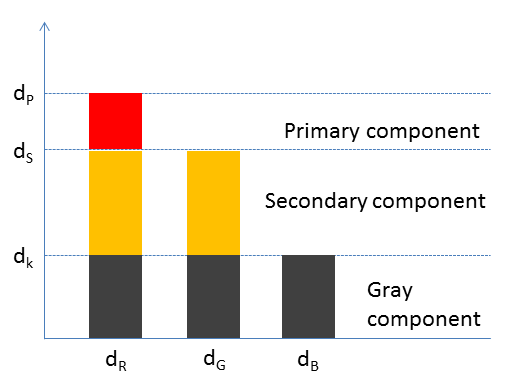
\includegraphics[width=0.6\columnwidth]{03_Rgb2XYZDisplayModule/images/psk_fact.png}
\end{tabular}
\end{center}
\caption{Construction of a PSK Factorization.}\label{PSKFactorisation}
\end{figure}

We use this factorization to construct one color triplet. It consists in blending the colors present in this factorization. 
From this point of view the quantity which must be blended has to be known. 
For this reason some fictive digital input are defined: $d_{K}$, $d_{S}$ and $d_{P}$, as follow.\par

\begin{defi}[Fictive digital inputs]
The fictive digital inputs are sorted as follow : $d_{K}\leqslant d_{S}\leqslant d_{P}$.\\
The fictive digital inputs concord with the digital inputs : $\left\{d_{K},d_{S},d_{P}\right\}=\left\{d_{R},d_{G},d_{B}\right\}$.\par
\label{defifictiveddl}
\end{defi}

\begin{example}[Remark]
$K$ stands for the gray (like the letter K in the word black). $S$ and $P$ respectively stand for a secondary and a primary color (from the PSK Factorization).
\end{example}

\begin{example}
Let $C$ be the obtained color  with the following digital input: $d_{R}=128$, $d_{G}=25$ and $d_{B}=44$.\par
With $d_{G}\leqslant d_{B}\leqslant d_{R}$, the fictive digital input is defined by: $d_{K}=d_{G}=25$, $d_{S}=d_{B}=44$ and $d_{P}=d_{R}=128$.\par
Therefore, the secondary color for the PSK factorization is obtained by blending red and blue. So the secondary is magenta, and the primary color of the PSK factorization is red.\par
The PSK factorization is therefore $\left\{\text{Gray, Magenta, Red}\right\}$.
\end{example}

We construct the color by mixing the colors from the PSK factorization. 
The $XYZ$ value of the color is calculated with the addition of three terms: one per color from the masking basis.\par
The construction is summarized in the following formula (formula \ref{formcolconstr}).

\begin{formula}[Color constructions]
$
\begin{array}{cc}
\text{Conventional construction}&I\left(d_{R},d_{G},d_{B}\right)=I_{R}\left(d_{R}\right)+I_{G}\left(d_{G}\right)+I_{B}\left(d_{B}\right)\\
\text{Masking construction}&I\left(d_{R},d_{G},d_{B}\right)=I_{K}\left(d_{K}\right)+\left[I_{S}\left(d_{S}\right)-I_{S}\left(d_{K}\right)\right]+\left[I_{P}\left(d_{P}\right)-I_{P}\left(d_{S}\right)\right]\\
\end{array}
$\par
\label{formcolconstr}
\end{formula}

By introducing $I_{S}$ and $I_{K}$ channel interactions can be considered. 
The masking construction is therefore more accurate than the conventional construction which does not take into account the channel interaction. $I\left(d_{R},d_{G},d_{B}\right)$ for the masking construction is approximated by $J\left(d_{R},d_{G},d_{B}\right)$ defined as follow: \par

\begin{formula}[Color approximation]\label{form_approx}
$
J\left(d_{R},d_{G},d_{B}\right)=J_{K}\left(d_{K}\right)+\left[J_{S}\left(d_{S}\right)-J_{S}\left(d_{K}\right)\right]+\left[J_{P}\left(d_{P}\right)-J_{P}\left(d_{S}\right)\right]
$\par
\label{formcolapprox}
\end{formula}

\subsubsection{The masking model in practice}

\paragraph{Data processing}
A Principal Component Analysis  (PCA) is applied on the measured XYZ values of each channel ($R, G, B, C, Y, M, K$). 
Therefore a single vector, $I_{PCA,i}$ stands for each channel ($I_R, I_G, I_B, I_C, I_Y, I_M, I_{K})$). 
So for each channel, the XYZ triplet values can be processed like scalar values. 
It is summarized in the following definition.\par

\begin{defi}[Approximated color curves]
Let $i$ be a color (R, G, B, C, Y, M, C, K).\par
$\forall ddl\in\left[0,d\right]$, $I_{i}\left(ddl\right)$ is approximated by $J_{i}\left(ddl\right)$ defined as follow.\\
\begin{center}
$J_{i}\left(ddl\right)=c_{i}\left(ddl\right)I_{PCA,i}+I\left(0,0,0\right)$.\par
\end{center}
where $J$, $I_{PCA}$ and $I$ correspond to vectors with size (3,1),
where $c_{i}$ is a scalar function.\par
\label{defiapproxcolorcurves}
\end{defi}

The color construction defined in the formula \ref{formcolconstr} can be therefore written as a matrix by using a masking transfer matrix form as follow:

\begin{defi}[Masking transfer matrix]
Let $\mathscr{B}=\left(P,S,K\right)$ be a masking basis.
The masking transfer matrix associated to $\mathscr{B}$ is the matrix $M_{\mathscr{B}}:=\left(I_{PCA,P}\mid I_{PCA,S}\mid I_{PCA,K}\right)$
\end{defi}

The development of the defined masking color construction in formula \ref{formcolconstr} is: 


\begin{formula}[Development of the color construction, step 1]
$J\left(d_{R},d_{G},d_{B}\right)=J_{K}\left(d_{K}\right)+\left[J_{S}\left(d_{S}\right)-J_{S}\left(d_{K}\right)\right]+\left[J_{P}\left(d_{P}\right)-J_{P}\left(d_{S}\right)\right]$
\label{form_dev_col_const}
\end{formula}
where $J_{K,S,P}$ is given by definition \ref{defiapproxcolorcurves}.\par

By injecting $J_{i}$ from definition \ref{defiapproxcolorcurves} in formula \ref{form_dev_col_const}, the following formula is obtained (formula \ref{form_dev_col_const2}):

\begin{formula}[Development of the color construction, step 2]
$\begin{array}{ll}
J\left(d_{R},d_{G},d_{B}\right)=&c_{K}\left(d_K\right)I_{PCA,K}+I\left(0,0,0\right)+\cdots\\
&\left[\left(c_{S}\left(d_S\right)I_{PCA,S}+I\left(0,0,0\right)\right)-(c_{S}\left(d_K\right)I_{PCA,S}+I\left(0,0,0\right))\right]+\cdots\\
&\left[\left(c_{P}\left(d_P\right)I_{PCA,P}+I\left(0,0,0\right)\right)-(c_{P}\left(d_S\right)I_{PCA,P}+I\left(0,0,0\right))\right]\\
\end{array}$
\label{form_dev_col_const2}
\end{formula}

\begin{formula}[Development of the color construction, step 3]
$
\vectorPage{X}{Y}{Z}\left(d_{R},d_{G},d_{B}\right)=c_{K}\left(d_K\right)\vectorPage{X_{PCA,K}}{Y_{PCA,K}}{Z_{PCA,K}}+I\left(0,0,0\right)+\cdots$\\$
\left[\left(c_{S}\left(d_S\right)\vectorPage{X_{PCA,S}}{Y_{PCA,S}}{Z_{PCA,S}}+I\left(0,0,0\right)\right)-\left(c_{S}\left(d_K\right)\vectorPage{X_{PCA,S}}{Y_{PCA,S}}{Z_{PCA,S}}+I\left(0,0,0\right)\right)\right]+\cdots$\\$
\left[\left(c_{P}\left(d_P\right)\vectorPage{X_{PCA,P}}{Y_{PCA,P}}{Z_{PCA,P}}+I\left(0,0,0\right)\right)-\left(c_{P}\left(d_S\right)\vectorPage{X_{PCA,P}}{Y_{PCA,P}}{Z_{PCA,P}}+I\left(0,0,0\right)\right)\right]
$
\label{form_dev_col_const3}
\end{formula}


\begin{formula}[The matrix $M_{\mathscr{B}}$, step 4]
$M_{\mathscr{B}} = \matrixcoeff{X_{PCA,P}}{Y_{PCA,P}}{Z_{PCA,P}}{X_{PCA,S}}{Y_{PCA,S}}{Z_{PCA,S}}{X_{PCA,K}}{Y_{PCA,K}}{Z_{PCA,K}}$
\label{form_dev_col_const4}
\end{formula}

\begin{formula}[Development of the color construction, step 5]

$I\left(d_{R},d_{G},d_{B}\right) =\matrixcoeff{X_{PCA,P}}{Y_{PCA,P}}{Z_{PCA,P}}{X_{PCA,S}}{Y_{PCA,S}}{Z_{PCA,S}}{X_{PCA,K}}{Y_{PCA,K}}{Z_{PCA,K}}\vectorPage{c_{p}\left(d_{p}\right)-c_{p}\left(d_{s}\right)}{c_{s}\left(d_{s}\right)-c_{s}\left(d_{K}\right)}{c_{K}\left(d_{K}\right)}+I\left(0,0,0\right)$
\label{form_dev_col_const5}
\end{formula}

In formula \ref{form_dev_col_const4} and \ref{form_dev_col_const5}, the matrix $M_{\mathscr{B}}$ corresponds to the new primary, secondary and gray components resulting from the principal component analysis. The 3 column vectors are unitary vectors. The coefficient's vector corresponds then to a norm and therefore to color intensity in the new basis.

\begin{prop}[Matrix writing of the color construction]
Let $\mathscr{B}$ be the masking basis associated to the color construction.\par
$I\left(d_{R},d_{G},d_{B}\right) =M_{\mathscr{B}}\vectorPage{c_{p}\left(d_{p}\right)-c_{p}\left(d_{s}\right)}{c_{s}\left(d_{s}\right)-c_{s}\left(d_{K}\right)}{c_{K}\left(d_{K}\right)}+I\left(0,0,0\right)$. 
\end{prop}

The three axes of the principal component analysis form an orthonormal basis. Therefore the scalar functions $c_{i}$ can be calculated as follow.

\begin{prop}[$c_{i}$ values]
Let $i$ be a color (R, G, B, C, Y, M, Gr) and let $c_{i}$ be the scalar function defined in definition \ref{defiapproxcolorcurves}.\par
$\forall ddl\in\left[0,d\right]$, $c_{i}\left(ddl\right)=\scalar{\left[J_{i}\left(ddl\right)-I\left(0,0,0\right)\right]}{I_{PCA,i}}$ .\par
\end{prop}
\begin{proof}
It is the calculation of an orthonormal factorization. 
\end{proof}

Color intensities must be expressed in the new basis, it is a norm and therefore it does correspond to the norm of the projected original color vector to the new axis.

So, by using the last proposal, the $c_{i}\left(ddl\right)$ are calculated thanks to the measured data (cf curve on the figure \ref{fig_cr_dr}). 

\begin{figure}[!h]
\begin{center}
\begin{tabular}{c}
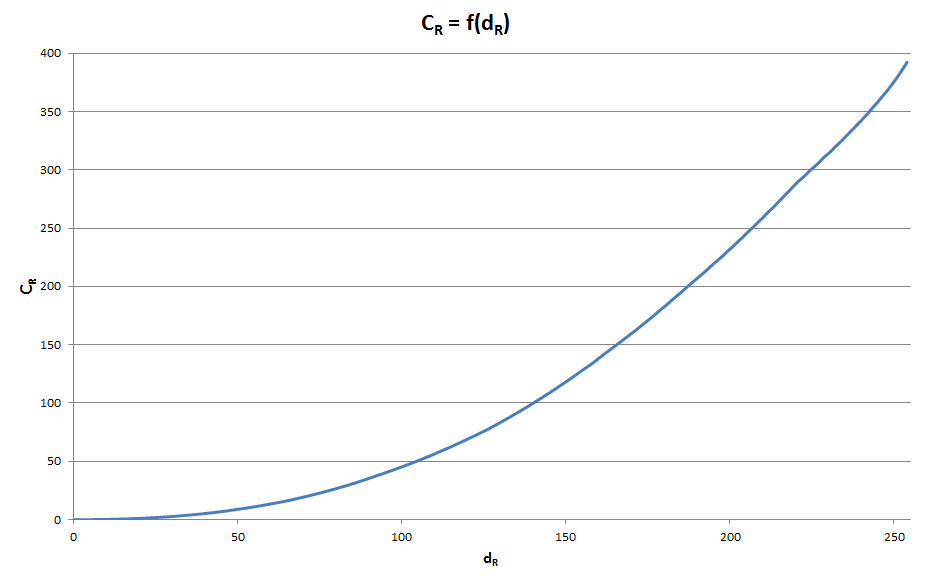
\includegraphics[width=0.6\columnwidth]{03_Rgb2XYZDisplayModule/images/cr_dr.png}
\end{tabular}
\end{center}
\caption{Coefficient of the first principal component for red.}\label{fig_cr_dr}
\end{figure}

The measured input values are limited. We only have $2^n$ input values per primary, secondary and gray curve. We need floating point digital input values. Therefore, simple linear interpolation (simple spline case) is used for calculating the $c_{i}$ values for any arbitrary digital input.\par

To use this theory and to calculate the associated digital input to any XYZ arbitrary values, reciprocal functions of the $c_{i}$ must be found. The following theorem proves the existence of these reciprocal functions.\par

\begin{theo}[Bijectivity of the $c_{i}$]
Let $i$ be a color (R, G, B, C, Y, M, Gr) and let $c_{i}$ be the scalar function defined in definition \ref{defiapproxcolorcurves}.\par
$c_{i}$ is a bijective function.
\end{theo}
\begin{proof}
$X$, $Y$ and $Z$ are increasing continuous functions of the digital inputs.
So the $c_{i}$ functions are also increasing and continuous.
So, using the bijection theorem, the $c_{i}$ functions are bijective. 
\end{proof}


In the two next subsections, the processing of the measures is supposed to have been made. 
So, the 7 $I_{PCAi}$ vectors and the $c_{i}$ functions (as their reverse functions) are supposed to be known.

\paragraph{Phases for the conversion from RGB to XYZ}
In this subsection, the conversion phases from any arbitrary digital input triplet values (in float) to XYZ triplet values are described.\par
Let $d_{R}$, $d_{G}$ and $d_{B}$ be the three arbitrary digital inputs.\par
First of all, we calculate the fictive digital inputs, $d_{P}$, $d_{S}$ and $d_{K}$ as given in definition \ref{defifictiveddl}.\par
Secondly we calculate the PSK factorization (called $\mathscr{B}$) of the color as given in definition \ref{defiPSKfactor}.\par
We calculate thirdly the masking transfer matrix, $M_{\mathscr{B}}$, and the associated coefficients $c_{i}\left(d_{i}\right)$.\par
Finally the resulting triplet $J\left(d_{R},d_{G},d_{B}\right)$ or ($X$,$Y$,$Z$) is calculated.\par


\subsubsection{Modified Masking Model}

The generic principle of the modified masking model does not differ too much compared to the masking model \cite{Tam02}. 

\paragraph{Conversion from RGB to XYZ}

The realized approximation given in definition \ref{defiapproxcolorcurves} is not effective since the deviation from linearity is very large. 

The common method described in \cite{Tam02} consists of including the second axis of the principal component analysis.
So the approximation of the color of the formula \ref{formcolconstr} is transformed by the following definition:

\begin{defi}[Approximated color curves in the Modified Masking Model]
Let $i$ be a color (R, G, B, C, Y, M, C, Gr).\par
$\forall ddl\in\left[0,d\right]$, $I_{i}\left(ddl\right)$ is approximate by $J_{i}\left(ddl\right)$ defined as follow.\\
\begin{center}
$J_{i}\left(ddl\right)=I\left(0,0,0\right)+c_{i,1}\left(ddl\right)I_{PCA,i,1}+{\bf c_{i,2}\left(ddl\right)I_{PCA,i,2}}$\par
\end{center}
\end{defi}

Using the same process than in the masking model, the value of the functions $c_{i,j}$ can be calculated and the value of $I\left(d_{R},d_{G},d_{B}\right)$ can be approximated by $I\left(d_{R},d_{G},d_{B}\right)$ calculated like in the masking model.\par
It is also possible to use this model to calculate the XYZ value associated to the digital input. 

The matrix $M_{\mathscr{B}}$ for the modified masking model is:

\begin{formula}[The matrix $M_{\mathscr{B}}$ for the modified masking model]
$M_{\mathscr{B}} = \left(\begin{array}{cccccc} 
X_{PCA,P,1} & X_{PCA,S,1} & X_{PCA,K,1} & X_{PCA,P,2} & X_{PCA,S,2} & X_{PCA,K,2}\\
Y_{PCA,P,1} & Y_{PCA,S,1} & Y_{PCA,K,1} & Y_{PCA,P,2} & Y_{PCA,S,2} & Y_{PCA,K,2}\\
Z_{PCA,P,1} & Z_{PCA,S,1} & Z_{PCA,K,1} & Z_{PCA,P,2} & Z_{PCA,S,2} & Z_{PCA,K,2}\\
\end{array} \right)$
\label{form_mask_model}
\end{formula}

The color construction for the modified masking model is:

\begin{formula}[Color construction]
$I\left(d_{R},d_{G},d_{B}\right) = \\ \left(\begin{array}{cccccc} 
X_{PCA,P,1} & X_{PCA,S,1} & X_{PCA,K,1} & X_{PCA,P,2} & X_{PCA,S,2} & X_{PCA,K,2}\\
Y_{PCA,P,1} & Y_{PCA,S,1} & Y_{PCA,K,1} & Y_{PCA,P,2} & Y_{PCA,S,2} & Y_{PCA,K,2}\\
Z_{PCA,P,1} & Z_{PCA,S,1} & Z_{PCA,K,1} & Z_{PCA,P,2} & Z_{PCA,S,2} & Z_{PCA,K,2}\\
\end{array} \right)\left(\begin{array}{c}
c_{P,1}\left(d_{P}\right)-c_{P,1}\left(d_{S}\right)\\
c_{P,1}\left(d_{S}\right)-c_{S,1}\left(d_{K}\right)\\
c_{K,1}\left(d_{K}\right)\\
c_{P,2}\left(d_{P}\right)-c_{P,2}\left(d_{S}\right)\\
c_{S,2}\left(d_{S}\right)-c_{S,2}\left(d_{K}\right)\\
c_{K,2}\left(d_{K}\right)\\
\end{array} \right)\\
+I\left(0,0,0\right)$
\label{form_col_const_mask_model}
\end{formula}


\section{Module: SaveFrameTXTModule}

This module saves a component in a txt file.

\subsection{Parameter: "Filename"}

This parameter is the path and filename of the output file without the extension ".txt". The extension is automatically generated.

\subsection{Parameter: "ComponentToWrite"}

This parameter selections the component to save. The module "SequenceRawGeneratorModule" creates a component with the index "0". The module "Rgb2XYZDisplayModule" creates a component with the index "1". The module "SaveFrameTxtModule" does not create any component.

Therefore if this parameter has the value "1", it will save the component of the module "Apply3x1DLutModule".

\subsection{Parameter: "FrameToWrite"}
This parameter selections the frame to save. If the value is "-1" then all frames will be saved.

\subsection{Parameter: "ChannelToWrite"}

This parameter selections the channel to save, in case of RGB by instance, three channels can be saved. If the value is "-1" then all channels will be saved.

The filename is given as input and an extension will be automatically generated with the extension ".txt".

The generated file can be simply edited or imported as "txt image" with ImageJ. 

\section{Module: SaveFrameRAWModule}

This module saves a component in a binary file.

\subsection{Parameter: "Filename"}

This parameter is the path and filename of the output file without the extension ".raw".

\subsection{Parameter: "ComponentToWrite"}

This parameter selections the component to save. The module "SequenceRawGeneratorModule" creates a component with the index "0". The module "Rgb2XYZDisplayModule" creates a component with the index "1". The module "SaveFrameRawModule" does not create any component.

Therefore if this parameter has the value "1", it will save the component of the module "SRgbDisplayModule".

\subsection{Parameter: "FrameToWrite"}
This parameter selections the frame to save. If the value is "-1" then all frames will be saved.

\subsection{Parameter: "ChannelToWrite"}

This parameter selections the channel to save, in case of RGB by instance, three channels can be saved. If the value is "-1" then all channels will be saved.

The filename is given as input and a filename extension will automatically generated with the extension ".raw".

An initialization txt file is automatically generated with the parameter to give for manipulating the raw file or open with ImageJ by instance:

SequenceRawGeneratorModule:

\lstset{language=Scilab}
\begin{lstlisting}
file name: ./output/sRGB
width: 64
height: 64
type imageJ: 32-bit Unsigned
\end{lstlisting}

Rgb2XYZDisplayModule:

\lstset{language=Scilab}
\begin{lstlisting}
file name: ./output/sRGB2XYZD50
width: 64
height: 64
type imageJ: 32-bit Real
\end{lstlisting}

The filename uses the filename given as input parameter and adds the suffix "\_description\_raw" before the extension ".raw".
